\documentclass[handout]{beamer}
\definecolor{lmu@green}{rgb}{0,0.58,0.25} % use structure theme to change
\definecolor{lmu@darkgreen}{rgb}{0,0.4,0.12} % use structure theme to change
% Uncomment the following for handouts.
%\documentclass[handout]{beamer}
\usepackage[utf8x]{inputenc}
\usepackage{amsmath,amsfonts,amssymb}
\setbeamertemplate{navigation symbols}{}

\usetheme{LMU}
\usecolortheme{lmu}
\useinnertheme{lmu}
\useoutertheme{lmu}


% Python listing setup

\usepackage{color}
\usepackage[procnames]{listings}
\usepackage{textcomp}
\usepackage{setspace}
\usepackage[]{xcolor}
\definecolor{gray}{gray}{0.5}
\definecolor{green}{rgb}{0,0.5,0}
\definecolor{lightgreen}{rgb}{0,0.7,0}
\definecolor{purple}{rgb}{0.5,0,0.5}
\definecolor{darkred}{rgb}{0.7,0,0}

\lstnewenvironment{python}[1][]{
\lstset{
% Escape with funnyeyes.
escapeinside={(*@}{@*)},
language=python,
basicstyle=\ttfamily\small,
stringstyle=\color{green},
showstringspaces=false,
alsoletter={1234567890},
otherkeywords={\ , \}, \{},
keywordstyle=\color{blue},
emph={access,and,as,break,class,continue,def,del,elif,else,%
except,exec,finally,for,from,global,if,import,in, is,%
lambda,not,or,pass,print,raise,return,try,while,assert},
emphstyle=\color{orange}\bfseries,
emph={[2]self},
emphstyle=[2]\color{gray},
emph={[4]ArithmeticError,AssertionError,AttributeError,BaseException,%
DeprecationWarning,EOFError,Ellipsis,EnvironmentError,Exception,%
False,FloatingPointError,FutureWarning,GeneratorExit,IOError,%
ImportError,ImportWarning,IndentationError,IndexError,KeyError,%
KeyboardInterrupt,LookupError,MemoryError,NameError,None,%
NotImplemented,NotImplementedError,OSError,OverflowError,%
PendingDeprecationWarning,ReferenceError,RuntimeError,RuntimeWarning,%
StandardError,StopIteration,SyntaxError,SyntaxWarning,SystemError,%
SystemExit,TabError,True,TypeError,UnboundLocalError,UnicodeDecodeError,%
UnicodeEncodeError,UnicodeError,UnicodeTranslateError,UnicodeWarning,%
UserWarning,ValueError,Warning,ZeroDivisionError,abs,all,any,apply,%
basestring,bool,buffer,callable,chr,classmethod,cmp,coerce,compile,%
complex,copyright,credits,delattr,dict,dir,divmod,enumerate,eval,%
execfile,exit,file,filter,float,frozenset,getattr,globals,hasattr,%
hash,help,hex,id,input,int,intern,isinstance,issubclass,iter,len,%
license,list,locals,long,map,max,min,object,oct,open,ord,pow,property,%
quit,range,raw_input,reduce,reload,repr,reversed,round,set,setattr,%
slice,sorted,staticmethod,str,sum,super,tuple,type,unichr,unicode,%
vars,xrange,zip},
emphstyle=[4]\color{purple}\bfseries,
upquote=true,
morecomment=[s][\color{lightgreen}]{"""}{"""},
commentstyle=\color{red}\slshape,
literate={>>>}{\bfseries{\textcolor{darkred}{>{>}>}}}3%
         {...}{{\textcolor{gray}{...}}}3,
procnamekeys={def,class},
procnamestyle=\color{blue}\textbf,
framexleftmargin=1mm, framextopmargin=1mm,
rulesepcolor=\color{blue},#1
}}{}


% -----------------------------------------------------------------------------
%
%\newtheorem{definition}{Definition}
\newcommand{\foot}[1]{_{\mbox{\footnotesize #1}}}
\newcommand{\head}[1]{^{\mbox{\footnotesize #1}}}
%
%
\newcommand{\ones}{\mathbb{I}}
\newcommand{\nat}{\mathbb{N}}
\newcommand{\real}{\mathbb{R}}
\newcommand{\ganz}{\mathbb{Z}}
%
%
\newcommand{\RRE}{\mbox{RRE}}
\newcommand{\nnz}[1]{\mbox{nnz}(#1)}
\newlength{\Hoehe}
\renewcommand{\vec}[1]{#1}
\newlength{\GLaenge}
\setlength{\GLaenge}{3.5cm}
%
%
\definecolor{MyGrey}{gray}{0.45}
\def\bstheta{\boldsymbol{\theta}}
\def\bsalpha{\boldsymbol{\alpha}}
\def\bsk{\boldsymbol{k}}
\def\bsx{\boldsymbol{x}}
\def\bsh{\boldsymbol{h}}
%
% Centred minipage environment
%
\newenvironment{cmpage}[1]{
\begin{center}
\begin{minipage}{#1\textwidth}}%
{\end{minipage}\end{center}}
%
%
\newcommand{\POS}{\color{blue}\item [\boldmath{$+$}]}
\newcommand{\NEG}{\color{red}\item [{\boldmath$-$}]}
\newcommand{\NTR}{\color{black}\item [$\circ$]}
\newcommand{\f}[1]{\mathfrak{#1}}
\newcommand{\old}{^{\mbox{\small \color{blue} old}}}
\newcommand{\new}{^{\mbox{\small \color{red} new}}}
\newcommand{\diag}[1]{\mbox{diag}\left(#1\right)}
%
%
\newcommand{\myBlank}{\textvisiblespace}
\newcommand{\noSpace}{\makebox[0pt]{\quad}}
%
% Old style colour commands
%
\newcommand{\CB}{\color{blue}}
\newcommand{\CR}{\color{red}}
\newcommand{\CG}{\color{green}}
\newcommand{\CC}{\color{cyan}}
%
\definecolor{myWhite}{rgb}{1.00,1.00,1.00}  % real white
\definecolor{myGrey}{rgb}{0.78,0.83,0.94}   % 'light grey blue'
\definecolor{myYellow}{rgb}{1.00,1.00,0.00} % yellow
\definecolor{myOrange}{rgb}{1.00,0.65,0.00} % orange
\definecolor{myCyan}{rgb}{0.00,1.00,1.00}   % cyan
%
% Some abbrevs for setting brief code parts
%
\newcommand{\ttA}{\mbox{\texttt{A}}}
\newcommand{\ttB}{\mbox{\texttt{B}}}
\newcommand{\ttC}{\mbox{\texttt{C}}}
\newcommand{\ttD}{\mbox{\texttt{D}}}
\newcommand{\code}[1]{\mbox{\texttt{#1}}}
\newcommand{\ccode}[1]{\cemphd{\texttt{#1}}}
%
% Commands for slides taken from 'Insides'
%
\newcommand{\rst}{\textcolor{emphcolora}{\ast}}
\newcommand{\bst}{\textcolor{emphcolorb}{\ast}}
%
%
%
\definecolor{textcolor} {rgb}{0,0,0}
\definecolor{decocolor} {rgb}{0,0,0}
\definecolor{emphcolora}{rgb}{1,0,0}              % pure red
\definecolor{emphcolorb}{rgb}{0,0,1}              % pure blue
\definecolor{emphcolorc}{cmyk}{0,1,0,0}           % pure magenta
%\definecolor{emphcolord}{cmyk}{0.64,0,0.95,0.20} % sort of green
\definecolor{emphcolord}{rgb}{0,0.4,0.12}         % same as lmu@darkgreen
\definecolor{emphcolore}{cmyk}{1,0,0,0}           % pure cyan
\definecolor{linkcolor} {rgb}{0,0,0}
%
% Commands emphasising text using color
%
\newcommand{\cempha}[1]{{\color{emphcolora}#1}}
\newcommand{\cemphb}[1]{{\color{emphcolorb}#1}}
\newcommand{\cemphc}[1]{{\color{emphcolorc}#1}}
\newcommand{\cemphd}[1]{{\color{emphcolord}#1}}
\newcommand{\cemphe}[1]{{\color{emphcolore}#1}}
\newcommand{\cemphf}[1]{{\color{decocolor}#1}}
% -----------------------------------------------------------------------------
% myColorBox
% -----------------------------------------------------------------------------
\setbeamercolor{myBoxColor}{fg=black,bg=white}
\setbeamercolor{myBoxColorHead}{fg=red,bg=white}
% \newenvironment{myColorBox}[2]{%
% \begin{beamerboxesrounded}[shadow=true,lower=myBoxColor,upper=myBoxColorHead,
% width=#1\textwidth]{#2}}%
% {\end{beamerboxesrounded}}
\newenvironment{myColorBox}[2]{%
\begin{cmpage}{#1}%
\begin{beamerboxesrounded}[shadow=true,lower=myBoxColor,upper=myBoxColorHead]%
{#2}}%
{\end{beamerboxesrounded}\end{cmpage}}
%
% -----------------------------------------------------------------------------
% Math Operators, alternate greek symbols and the like
% -----------------------------------------------------------------------------
\DeclareMathOperator{\grad}{grad}
\DeclareMathOperator{\mydiv}{div}
\DeclareMathOperator{\Grad}{grad}
\DeclareMathOperator{\Div}{div}
%\newcommand{\grad}{\mbox{grad}}
%\newcommand{\mydiv}{\mbox{div}}
\renewcommand{\rho}{\varrho}
%
% -----------------------------------------------------------------------------
% Some color defintions to be compatible with XFIG
% -----------------------------------------------------------------------------
%
\definecolor{XFIGgold}{rgb}{1.00,0.84,0.00}
\definecolor{XFIGltblue}{rgb}{0.53,0.81,1.00}
\definecolor{XFIGred}{rgb}{1.00,0.00,0.00}
% -----------------------------------------------------------------------------


\usepackage[T1]{fontenc}
\usepackage{lmodern}
\usepackage[scaled]{beramono}


% Meta information.
\title{ObsPy: A Python Toolbox for Seismology}
\subtitle{\tiny{Last Updated: April 2013}}
\author[L. Krischer]{Lion Krischer}
\date{}
\institute[LMU]{Ludwig-Maximilians-University in Munich\\ Department of Earth and Environmental Sciences\\ Geophysics}

\begin{document}

% Title page.
% Use \frame[plain]{\titlepage} for a title page without decorating elements.
\frame[plain]{\titlepage}



%%%%%%
% PYTHON SECTION

\begin{frame}[plain]

        \hspace{10ex}\textcolor{lmu@darkgreen}{\Large{1. Python}}

        \vspace{10ex}

        \hspace{10ex}\textcolor{lmu@darkgreen}{\Large{2. ObsPy}}
\end{frame}

\begin{frame}[plain]{Why use Python?}
    \begin{itemize}
        \item Easy \\ $\Rightarrow$ Learning curve similar to Matlab
        \item Free
        \item Runs everywhere
        \item Code should be a tool and work for you - not against you
    \end{itemize}
\end{frame}

\begin{frame}[plain]{Why use Python?}
    \begin{itemize}
        \item Open Source
        \item Cross-platform
        \item General purpose language (in contrast to other tools used in science)
        \item No need to compile
        \item Interactive shell
        \item Readability
        \item Speed
        \item ``Batteries included''
        \item Mature third party libraries
        \item Makes it easy to interact with existing C and Fortran code
    \end{itemize}
\end{frame}

\begin{frame}[plain]{Why use Python?}
    \begin{itemize}
        \item One of the most used programming languages
        \item Huge community outside of science \\ $\Rightarrow$ Tools and support widely available
        \item Used a lot in the web community \\ $\Rightarrow$ Will become more and more important
        \item Big support from the data analysis community
        \item Interesting new developments: pypy, blaze, numba, ipython, \dots
        \item Future proof
    \end{itemize}
\end{frame}



\begin{frame}[plain]{Must have third party libraries/tools}
    \begin{itemize}
        \item \textbf{NumPy/SciPy} - array and matrix structures, linear algebra routines, numerical optimization, random number generation, statistics routines, differential equation modeling, Fourier transforms and signal processing, image processing, sparse and masked arrays, spatial computation, and numerous other mathematical routines
        \item \textbf{matplotlib} - 2D (and limited 3D) plotting library which produces publication quality figures via a set of functions familiar to MATLAB users
        \item \textbf{basemap} - Maps
        \item \textbf{IPython} - Enhanced interactive shell, also provides a HTML notebook
        \item \textbf{lxml}, \textbf{PyQt}, \textbf{Pandas}, \textbf{pytables}, \textbf{SQLAlchemy} \dots
    \end{itemize}
\end{frame}


\begin{frame}[fragile, plain]
    \frametitle{Readable Syntax}

\begin{myColorBox}{0.8}{}
\begin{python}
>>> 3 in [1, 2, 3, 4, 5]
True
>>> "sub" in "substring"
True


>>> open_file = open("filename", "r")
>>> for line in open_file:
...     print line


>>> for i in [1, 2, 3, 4, 5]:
...   if i < 3:
...       print i,
...   else:
...       print i * 2,
1 2 6 8 10


\end{python}
\end{myColorBox}

\end{frame}

\begin{frame}[fragile, plain]
    \frametitle{''Batteries included''}
    \begin{itemize}
        \item Extensive standard libraries:
        \begin{itemize}
            \item \textbf{Powerful string handling}
            \item \textbf{Filesystem manipulation utitilties}
            \item Data Persistence
            \item Data Compression and Archiving
            \item Cryptographic Services
            \item \textbf{Internet Protocols and Data Handling}
            \item Structured Markup Processing Tools
            \item Development Tools
            \item Multithreading \& Multiprocessing
            \item \textbf{Regular expressions}
            \item Graphical User Interfaces with Tk
            \item ...
        \end{itemize}
    \end{itemize}
\end{frame}

\begin{frame}[fragile, plain]
    \frametitle{''Batteries included''}
    \begin{itemize}
        \item Well-documented
        \item Platform independent API, but optimized for each platform
        \item One place to look first for a proven solution
        \item Reuse instead of reinvent
    \end{itemize}
\end{frame}

\begin{frame}[fragile, plain]
    \frametitle{Speed}
    \begin{center}
    \Large{\textit{``Python is extremely slow and wastes memory!''}}
    \normalsize
    \end{center}
\end{frame}



\begin{frame}[fragile, plain]
    \frametitle{Implementation Time vs. Execution Time}
     \begin{itemize}
    	\item Python is designed for productivity
    	\pause
    	\item No compilation step
       \begin{itemize}
	    \item No compiler problems
	    \item No makefiles
	    \item No linker problems
	    \item Faster development cycles
        \end{itemize}
    	\pause
    	\item When execution speed matters:
        \begin{itemize}
    	    \item Use specialized modules
    	    \item Implement time critical parts in C/C++/Fortran/Cython
      	    \item Profile
      	    \item Use specialized JIT compiler (e.g. PyPy or Numba)
        \end{itemize}
        \item Python is fast enough in most cases.
        \item Otherwise choose the right tool!
    \end{itemize}
\end{frame}

\begin{frame}[fragile, plain]
    \frametitle{Language Interoperability}
    Python excels at gluing other languages together:
     \begin{itemize}
       \item \textbf{FORTRAN}: F2py - Fortran to Python interface generator (part of NumPy).
       \pause
       \item General \textbf{C} or \textbf{C++} libraries: Ctypes, Cython, or SWIG are three ways to interface them.
       \pause
       \item \textbf{R}: RPy - simple, robust Python interface to the R Programming Language. It can manage all kinds of R objects and can execute arbitrary R functions (including the graphic functions).
    \end{itemize}
     \begin{itemize}
       \item \textbf{Matlab}: The similarity of Matlab and NumPy/SciPy/matplotlib makes it very easy to transfer existing code. NumPy can directly read the files saved by Matlab.
    \end{itemize}
\end{frame}

\begin{frame}[plain]{IPython Console}
    \begin{center}
        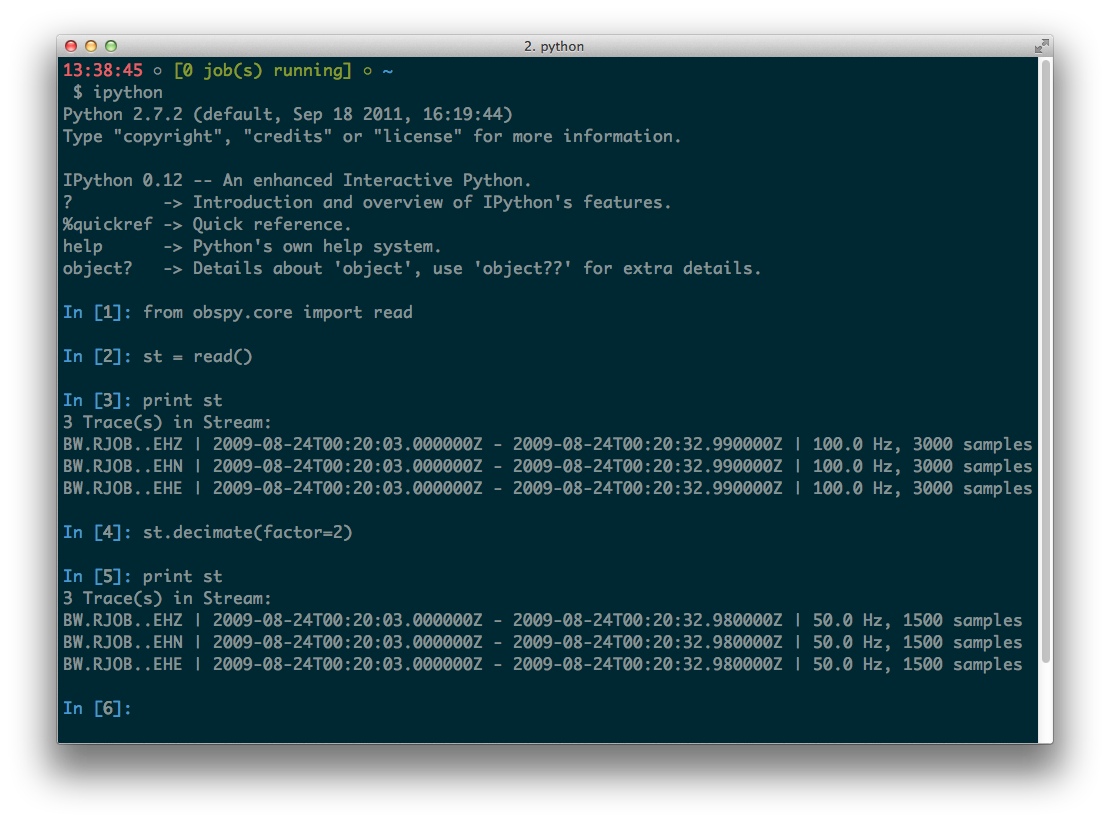
\includegraphics[height=0.94\paperheight]{images/ipy_screenshot.png}
    \end{center}
\end{frame}

\begin{frame}[plain]{IPython HTML Notebook}
    \begin{center}
        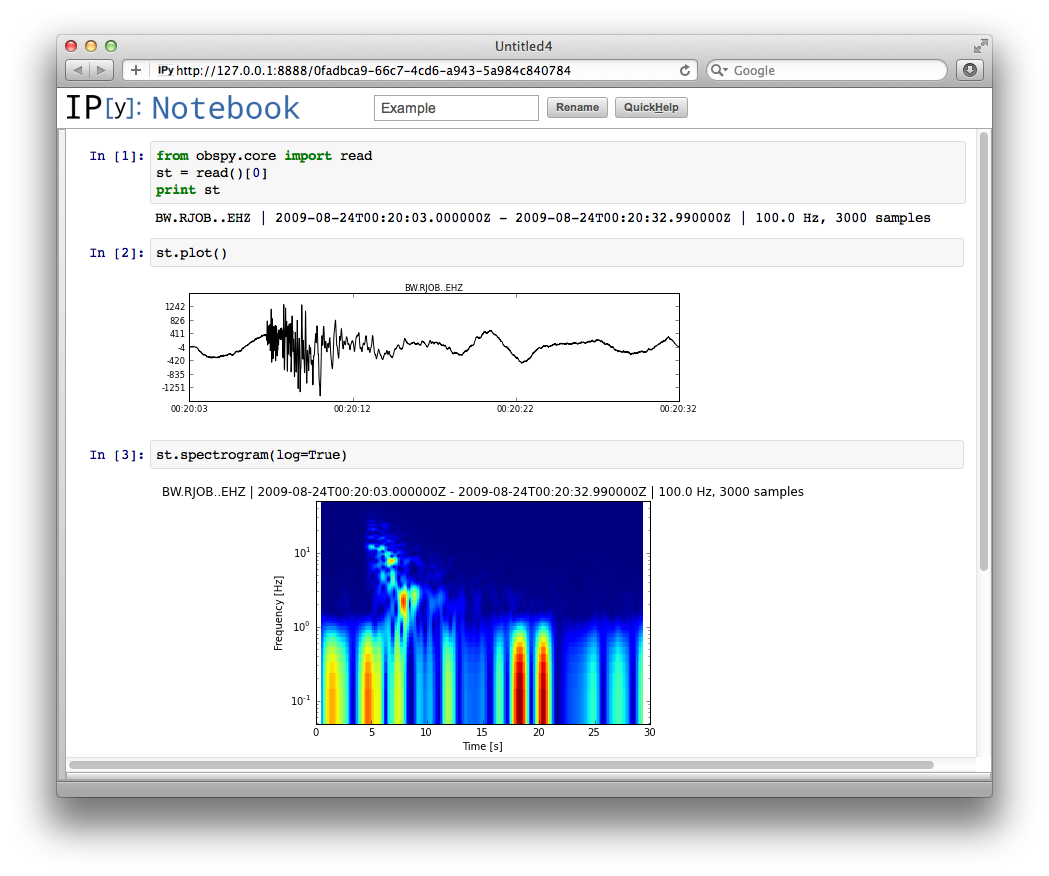
\includegraphics[height=0.95\paperheight]{images/ipy_notebook.png}
    \end{center}
\end{frame}



\begin{frame}[plain]
        \begin{center}
        \textcolor{lmu@darkgreen}{\Large{ObsPy}}
        \end{center}
\end{frame}

\begin{frame}[plain]{What is ObsPy and what can it do}
    A Python Toolbox for seismology/seismological observatories.

    \vspace{2em}

    The goal of the ObsPy project is to \textbf{facilitate rapid application development for seismology}.

    \vspace{3em}

    \large
    \begin{center}
        \textbf{https://www.obspy.org}
    \end{center}
\end{frame}


\begin{frame}[plain, fragile]{What is ObsPy and what can it do}
    \begin{itemize}
        \item In development since 2008
        \item 6 core developers
        \item Many more people contribute (currently around 25 people contributed code)
        \item Thoroughly unit tested
        \item Written in Python (performance critical parts are written in C)
        \item Uses well established libraries (libmseed, GSE\_UTI, \dots)
        \item Open source and cross platform
        \item Starts to get widely used in the community \\ $\Rightarrow$ Estimated active user base: > 5000
    \end{itemize}
\end{frame}

\begin{frame}[plain]
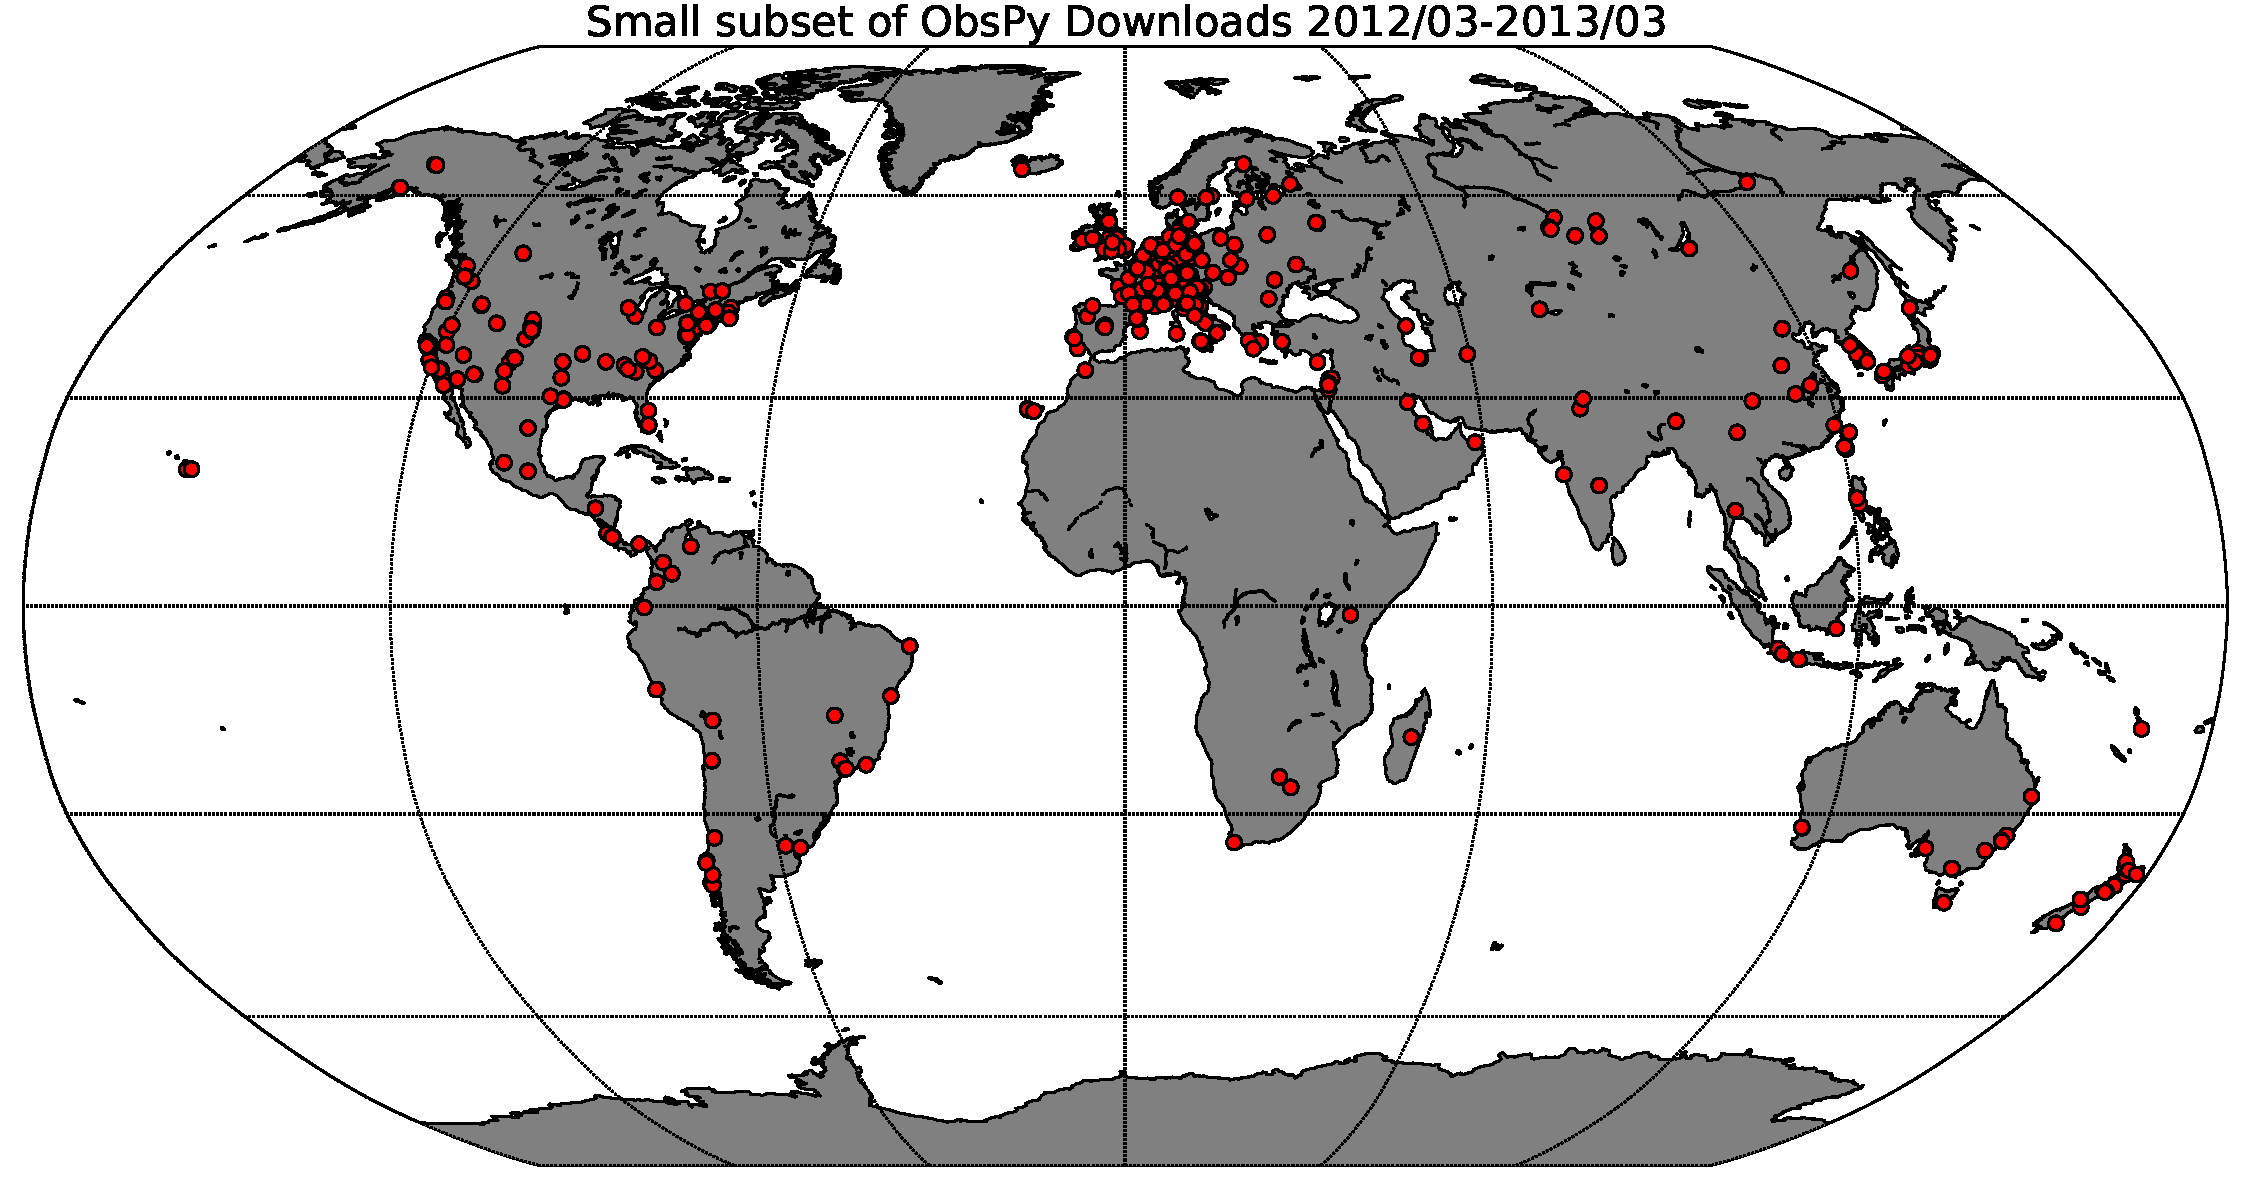
\includegraphics[width=\textwidth]{./Scripts/ObsPyUsers.pdf}
\end{frame}

\begin{frame}[plain]
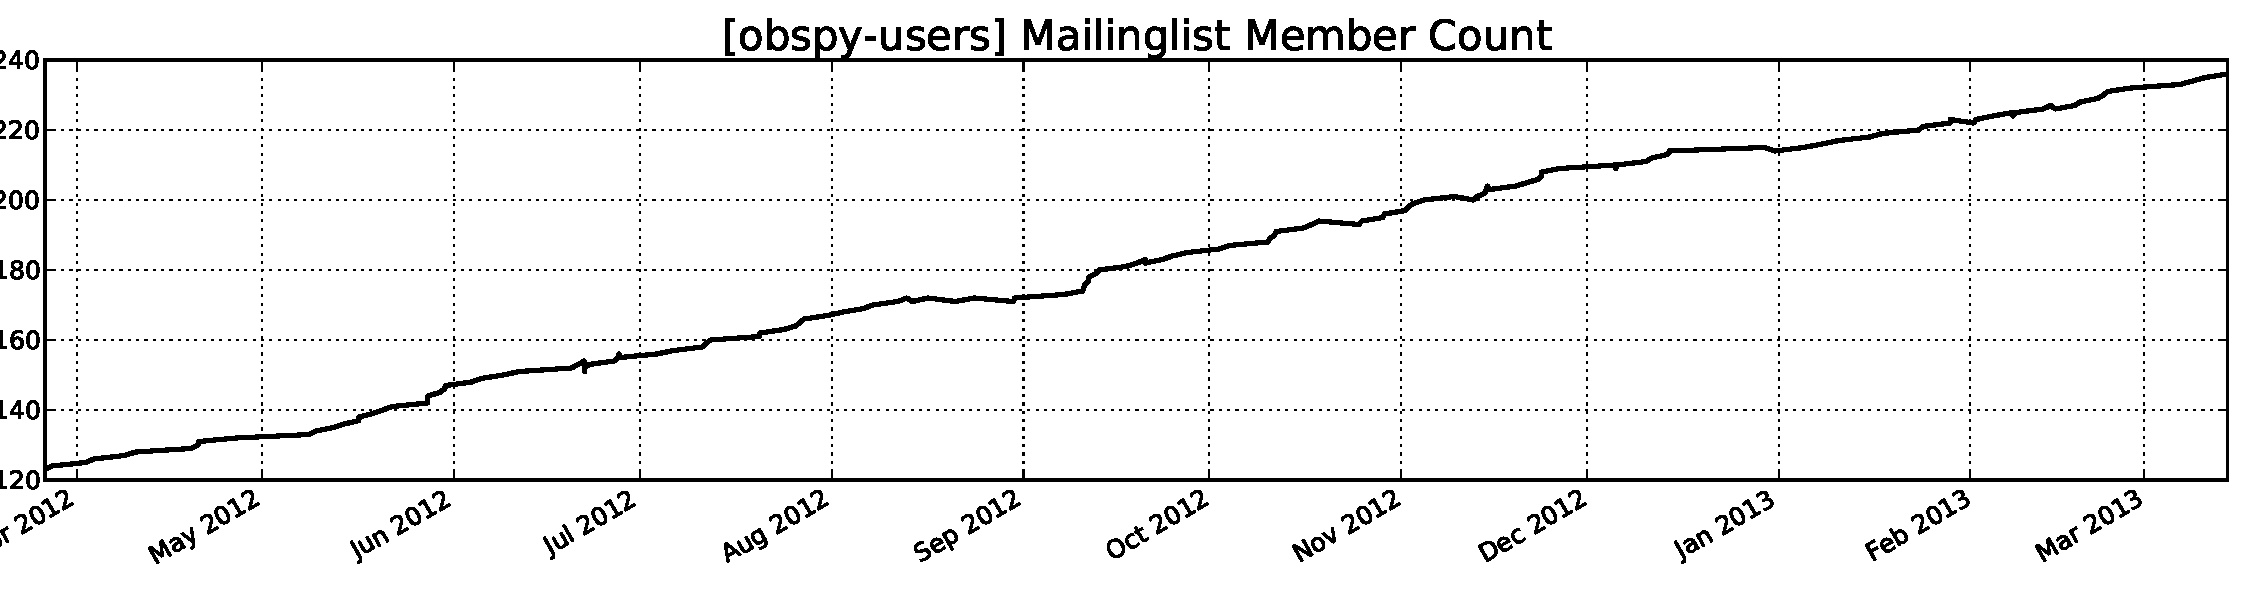
\includegraphics[width=\textwidth]{./Scripts/ObspyMailinglist.pdf}
\vspace{5ex}
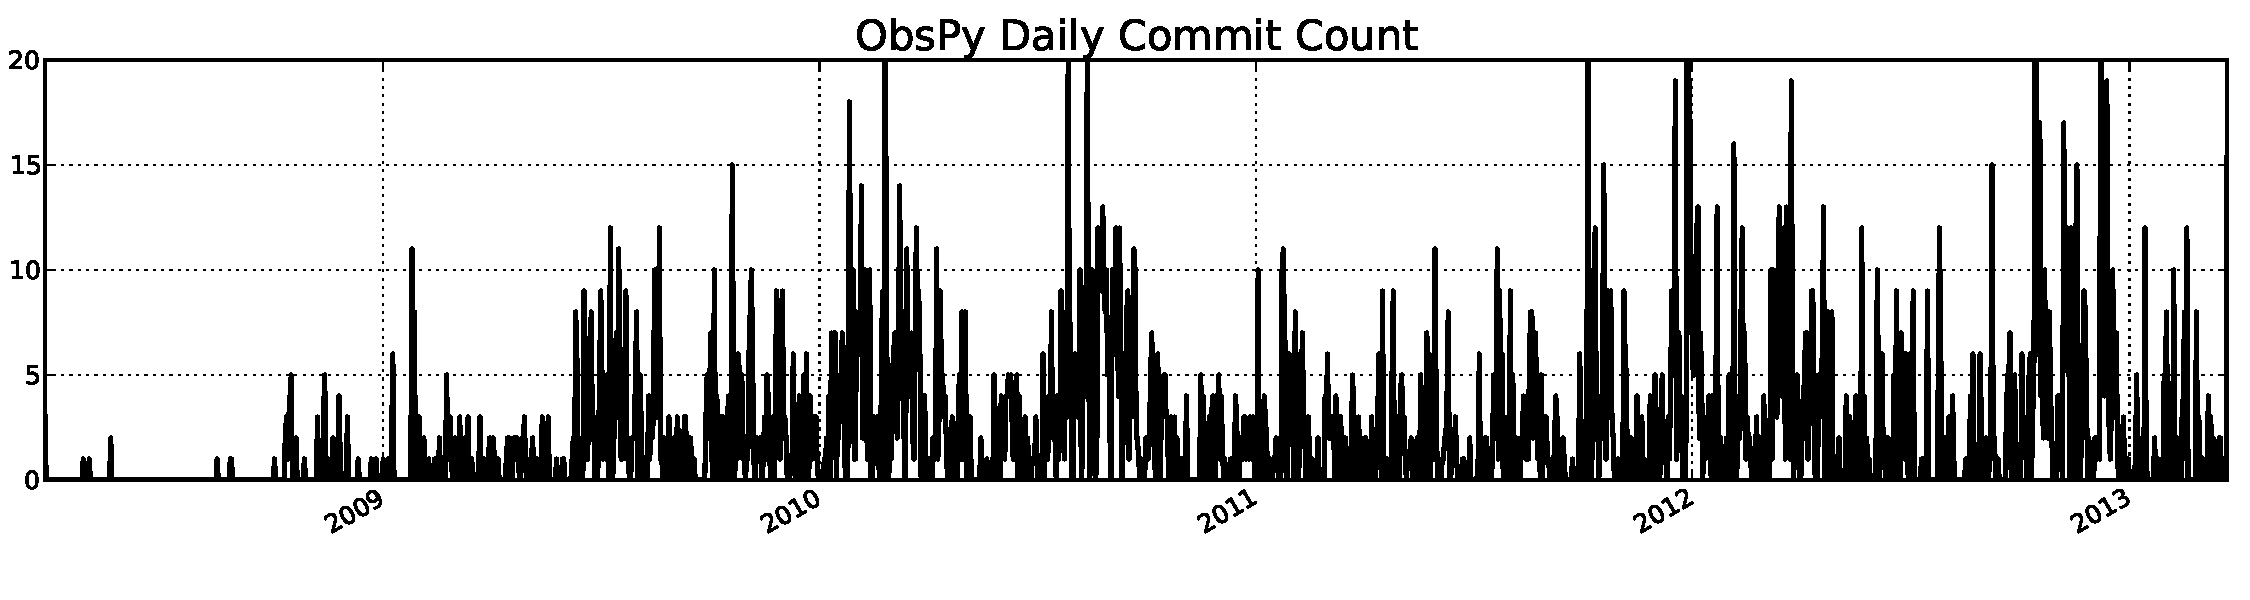
\includegraphics[width=\textwidth]{./Scripts/ObsPyDailyCommits.pdf}
\end{frame}


\begin{frame}[plain, fragile]{What is ObsPy and what can it do}
    \begin{itemize}
        \item \textbf{Read and write waveform data in various formats} (MiniSEED, SAC, GSE, SEG Y, \dots) with a unified interface.
        \item \textbf{Database and webservice access clients} for NERIES, IRIS DMC, ArcLink, SeisHub and Earthworm (experimental).
        \item \textbf{Many seismological signal processing routines} like filters, trigger, instrument correction, array analysis, beamforming, \dots
        \item \textbf{Support for inventory data} (SEED, XSEED, RESP and planned StationXML support)
        \item \textbf{Event data handling}
    \end{itemize}
    \begin{center}
        +
    \end{center}

    \begin{center}
        \textbf{The full power and flexibility of Python.}
    \end{center}

\end{frame}


\begin{frame}[plain, fragile]{Simple example - Reading a waveform file}
\begin{myColorBox}{0.95}{}

\begin{python}
>>> from obspy import read
>>> st = read("waveform.mseed")
>>> print st
1 Trace(s) in Stream:
BW.FURT..EHZ | 2010-01-04 ... | 200.0 Hz, 7204234 samples
\end{python}
\end{myColorBox}

\begin{itemize}
    \item Automatic file format detection.
    \item Always results in a Stream object.
    \item Raw data available as a numpy.ndarray.
\end{itemize}
\begin{myColorBox}{0.95}{}
\begin{python}
>>> st[0].data
array([-426, -400, ... , -489, -339], dtype=int32)
\end{python}
\end{myColorBox}
\end{frame}


\begin{frame}[plain, fragile]{Working with the waveform data.}
\begin{myColorBox}{0.95}{}

\begin{python}
>>> print st
1 Trace(s) in Stream:
BW.FURT..EHZ | 2010-01-05T ... | 200.0 Hz, 17280068 samples
>>> st.trim(endtime=st[0].stats.starttime + 3600)
>>> st.decimate(factor=2)
>>> st.filter("lowpass", freq=1.0)
>>> print st
BW.FURT..EHZ | 2010-01-05T ... | 100.0 Hz, 360001 samples
>>> st.plot()
\end{python}
\end{myColorBox}
\end{frame}



\begin{frame}[plain, fragile]{The resulting Stream object}
 \begin{itemize}
     \item A \textbf{Stream} object is a collection of \textbf{Trace} objects
     \item A \textbf{Trace} object is a single, continuous waveform data block
     \item Working with them is easy:
         \begin{itemize}
             \item \textbf{st.filter()} - Filter all attached traces.
             \item \textbf{st.trim()} - Cut all traces.
             \item \textbf{st.resample() / st.decimate()} - Change the sampling rate.
             \item \textbf{st.trigger()} - Run triggering algorithms.
             \item \textbf{st.plot() / st.spectrogram()} - Visualize the data.
             \item \textbf{st.simulate(), st.merge(), st.normalize(), st.detrend(), \dots}
         \end{itemize}
     \item A \textbf{Stream} object can also be exported to many formats making ObsPy a good tool for converting between different file formats.
\end{itemize}
\begin{myColorBox}{0.95}{}
\begin{python}
>>> st.write("output_file.sac", format="SAC")
\end{python}
\end{myColorBox}

\end{frame}


\begin{frame}[plain, fragile]{Handling time - The UTCDateTime class}
    \begin{itemize}
        \item All absolute time values are consistently handled with this class.
        \item No ambiguities, e.g. timezones, leap seconds, \dots
        \item Based on a high precision POSIX timestamp
        \item Easy usage:
\end{itemize}
\begin{myColorBox}{0.95}{}
\begin{python}
>>> from obspy import UTCDateTime
>>> time = UTCDateTime(2012, 9, 12, 8, 0, 0)
>>> one_hour_later = time + 3600

>>> UTCDateTime() - time
8078.097172
\end{python}
\end{myColorBox}

\end{frame}

\begin{frame}[fragile, plain]{Inventory Data}
    \begin{itemize}
        \item Can currently read/write/convert between SEED and XML-SEED.
        \item RESP file support.
        \item StationXML support is planned.
    \end{itemize}


\footnotesize
\begin{myColorBox}{0.95}{}
\begin{semiverbatim}
000001V 010009402.3121970,001,00:00:00.0000~2038,001,00:00:00.0000~
2009,037,04:32:41.0000~BayernNetz~~0110032002RJOB 000003RJOB 000008
...
\end{semiverbatim}
\end{myColorBox}

\large
\begin{center}
    $\Updownarrow$
\end{center}

\footnotesize


\begin{myColorBox}{0.95}{}
\begin{semiverbatim}
<?xml version='1.0' encoding='utf-8'?>
<xseed version="1.0">
  <volume_index_control_header>
    <volume_identifier blockette="010">
      <version_of_format>2.4</version_of_format>
      <logical_record_length>12</logical_record_length>
      <beginning_time>1970-01-01T00:00:00</beginning_time>
      <end_time>2038-01-01T00:00:00</end_time>
...
\end{semiverbatim}
\end{myColorBox}

\normalsize

\end{frame}

\begin{frame}[fragile, plain]{Inventory Data - Example usage}
\begin{myColorBox}{0.95}{}
\begin{python}
>>> from obspy.xseed import Parser
>>> p = Parser("dataless_SEED")
>>> print p
BW.FURT..EHZ | 2001-01-01T00:00:00.000000Z -
BW.FURT..EHN | 2001-01-01T00:00:00.000000Z -
BW.FURT..EHE | 2001-01-01T00:00:00.000000Z -
>>> p.getCoordinates("BW.FURT..EHZ")
{"elevation": 565.0, "latitude": 48.162899,
 "longitude": 11.2752}
>>> p.getPAZ("BW.FURT..EHZ")
{"digitizer_gain": 1677850.0,
 "gain": 1.0,
 "poles": [(-4.444+4.444j), (-4.444-4.444j), (-1.083+0j)],
 "seismometer_gain": 400.0,
 "sensitivity": 671140000.0,
 "zeros": [0j, 0j, 0j]}
\end{python}
\end{myColorBox}
\end{frame}


\begin{frame}[plain, fragile]{Events}
    \begin{itemize}
        \item Aims to get a unified interface with read and write support independent of the data source, similar to how the Stream and Trace classes handle waveform data.
        \item Modelled after QuakeML - currently supports QuakeML 1.2
    \end{itemize}
\begin{myColorBox}{0.95}{}
\begin{python}
>>> from obspy import readEvents
>>> url = "http://www.seismicportal.eu/services/..."
>>> catalog = readEvents(url)
>>> print catalog
99 Event(s) in Catalog:
2012-04-11T10:43:09.400000Z |  ... | 8.2 Mw | ...
2012-04-11T08:38:33.000000Z |  ... | 8.4 M  | ...
...
\end{python}
\end{myColorBox}
\end{frame}

\begin{frame}[plain, fragile]{The Catalog object}
    \begin{itemize}
        \item The Catalog object contains some convenience methods to make working with events easier.
        \item Events can be filtered with various keys.
    \end{itemize}
\begin{myColorBox}{0.95}{}
\begin{python}
>>> small_magnitude_events = cat.filter("magnitude <= 4.0")
\end{python}
\end{myColorBox}

    \begin{itemize}
        \item They can be plotted using the basemap module.
    \end{itemize}
\begin{myColorBox}{0.95}{}
\begin{python}
    >>> cat.plot()
\end{python}
\end{myColorBox}
    \begin{itemize}
        \item And they can be written.
    \end{itemize}
\begin{myColorBox}{0.95}{}
\begin{python}
>>> cat.write("modified_events.xml", format="quakeml")
\end{python}
\end{myColorBox}
\end{frame}


\begin{frame}[plain]
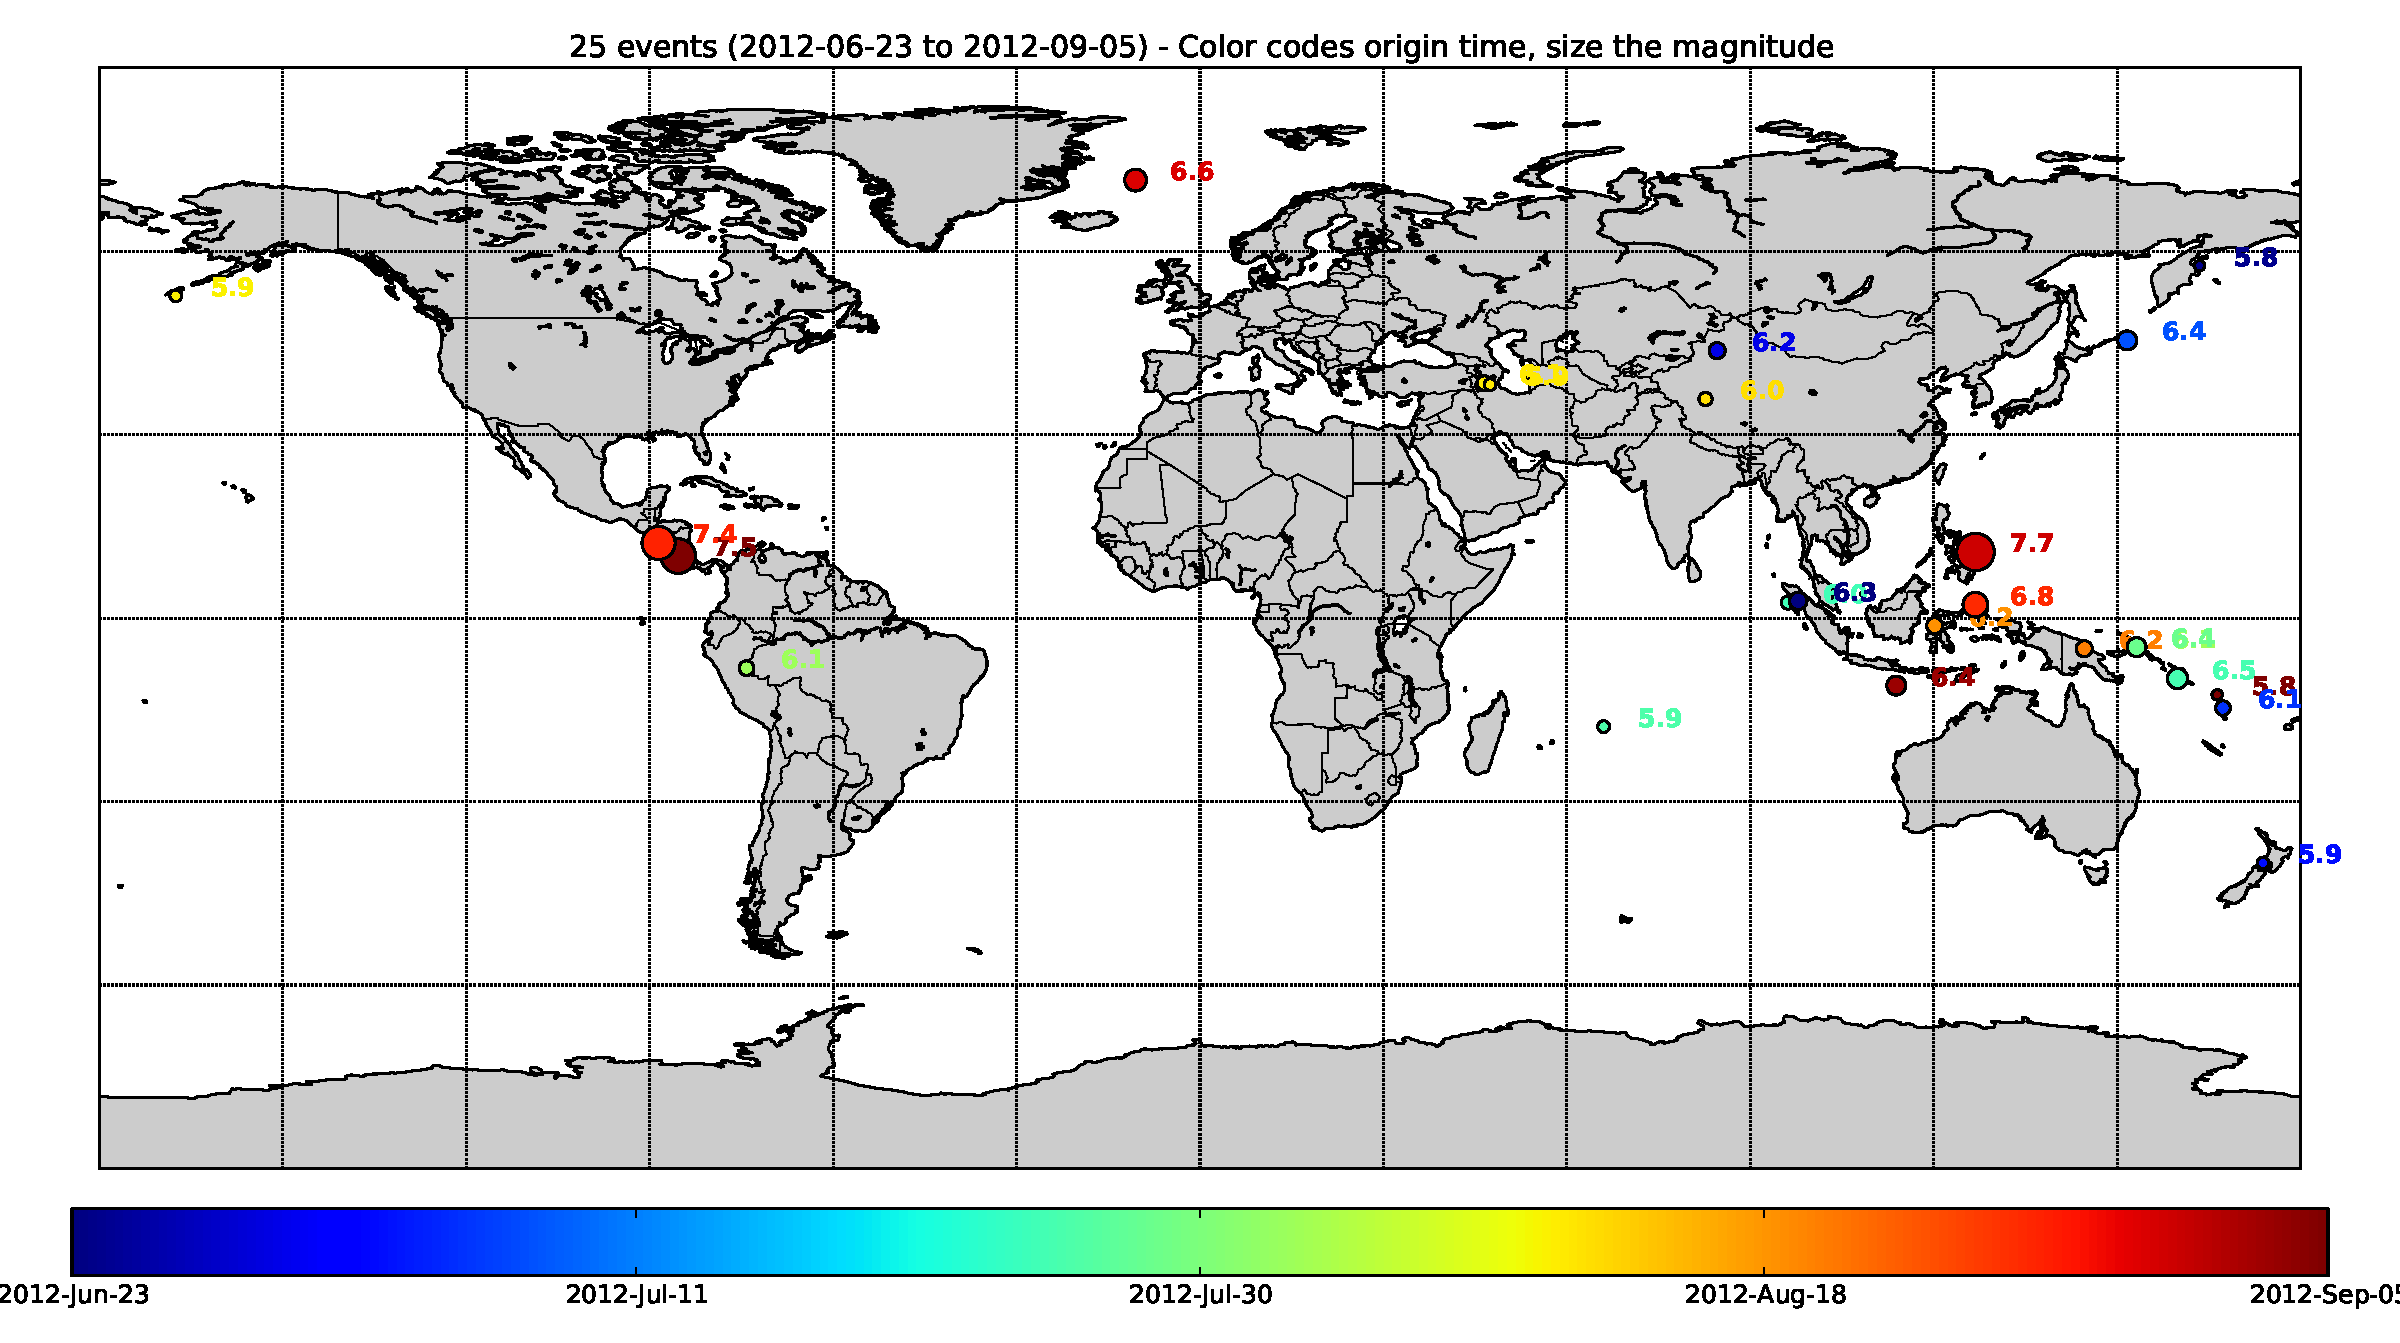
\includegraphics[width=\textwidth]{events.pdf}
\end{frame}


\begin{frame}[plain, fragile]{Clients - Getting waveform data from the web}
    Available for \textbf{NERIES}, \textbf{IRIS}, \textbf{ArcLink}, \textbf{SeisHub} and \textbf{Earthworm}.

\begin{myColorBox}{0.95}{}
\begin{python}
>>> from obspy.neries import Client
>>> from obspy import UTCDateTime
>>> client = Client(user="test@obspy.org")
>>> dt = UTCDateTime("2009-08-20 04:03:12")
>>> st = client.getWaveform("BW", "RJOB", "", "EH*", \
                            dt - 3, dt + 15)
>>> print st
3 Trace(s) in Stream:
BW.RJOB..EHN | 2009-08-20T04: ... | 200.0 Hz, 3601 samples
BW.RJOB..EHE | 2009-08-20T04: ... | 200.0 Hz, 3601 samples
BW.RJOB..EHZ | 2009-08-20T04: ... | 200.0 Hz, 3601 samples
\end{python}
\end{myColorBox}
\begin{itemize}
    \item Similar interfaces for the other clients.
    \item The returned object is the same as if read from a file.
\end{itemize}
\end{frame}


\begin{frame}[plain]{Clients - Retrieving other data}
    The webservices are not limited to retrieving waveform data. Depending on the client module used, the available data includes:
    \vspace{2em}
    \begin{itemize}
        \item Events information
        \item Inventory and response data
        \item Availability information
        \item \dots
    \end{itemize}
\end{frame}



\begin{frame}[plain, fragile]{}
    \begin{center}
        \textcolor{lmu@darkgreen}{\LARGE{obspy.signal - Signal Processing Routines}}
    \end{center}
\end{frame}


\begin{frame}[plain, fragile]{}

\footnotesize
\begin{verbatim}
sonic                      cfrequency                fem
array_transff_wavenumber   bwith                     fpm
array_transff_freqslowness domperiod                 em
relcalstack                logbankm                  pm
envelope                   logcep                    tpg
normEnvelope               sonogram                  rdct
centroid                   cosTaper                  fpg
instFreq                   c_sac_taper               eg
instBwith                  evalresp                  pg
xcorr                      cornFreq2Paz              plotTfMisfits
xcorr_3C                   pazToFreqResp             plotTfGofs
xcorr_max                  waterlevel                plotTfr
xcorrPickCorrection        specInv                   recSTALTA
simple                     seisSim                   carlSTATrig
bandpass                   paz2AmpValueOfFreqResp    classicSTALTA
bandstop                   estimateMagnitude         delayedSTALTA
lowpass                    estimateWoodAndersonA...  zDetect
highpass                   konnoOhmachiSmoothing     triggerOnset
envelope                   eigval                    pkBaer
remezFIR                   class PPSD                arPick
lowpassFIR                 rotate_NE_RT              plotTrigger
integerDecimation          rotate_ZNE_LQT            coincidenceTrigger
lowpassCheby2              rotate_LQT_ZNE            utlGeoKm
polarizationFilter         cwt                       utlLonLat
\end{verbatim}
\end{frame}


\begin{frame}[plain, fragile]{Complete Workflow Example}
\begin{myColorBox}{0.95}{}
\begin{python}
from obpsy import UTCDateTime
from obspy.arclink import Client()
client = Client()
t0 = UTCDateTime("2012-09-08 20:30:00")
# Download data and instrument response.
st = client.getWaveform ("NA", "SABA", "", "BHZ", \
    t0 - 900, t0 + 900)
paz = client.getPAZ ("NA", "SABA", "", "BHZ", t0 )
# Add a zero to convert to m (default is m/s)
paz["zeros"].append(0 + 0j)
st.simulate(paz_remove=paz)
# Apply highpass filters
st.filter("highpass",freq=0.005)
# Trim the signal to your needs
st.trim(t0 - 60, t0 + 60)
# Save and plot the deconvolved data
st.write("deconvolved_data", format="mseed")
st.plot()
\end{python}
\end{myColorBox}
\end{frame}


\begin{frame}[plain]{What's next?}
    \begin{itemize}
            \item \textbf{Getting more developers and external contributions} \\ $\Rightarrow$ We try to be as open as possible and very much encourage people to add to/modify our code basis
            \item Adding support for Python 3 (partially done)
            \item Support for StationXML (partially done)
            \item More powerful instrument correction module
            \item Suggestions? Let us know!
    \end{itemize}
\end{frame}


\begin{frame}[plain]{www.obspy.org}
    \begin{itemize}
        \item Documentation and extensive tutorial.
        \item Gallery to showcase some features.
        \item \textbf{mailing list} - subscribe for updates and discussions about the project.
        \item Source code repository and bug tracker.
        \item Automatic, daily running tests bots (https://tests.obspy.org)
        \item Get in touch!
    \end{itemize}

    \vspace{2em}

    \small
    \begin{itemize}
        \item Moritz Beyreuther et al. (2010) \textbf{ObsPy: A Python Toolbox for Seismology}, SRL, 81(3), 530-533
        \item Tobias Megies et al. (2011) \textbf{ObsPy – What can it do for data centers and observatories?} Annals Of Geophysics, 54(1), 47-58. doi:10.4401/ag-4838
    \end{itemize}
\end{frame}


\begin{frame}[plain]
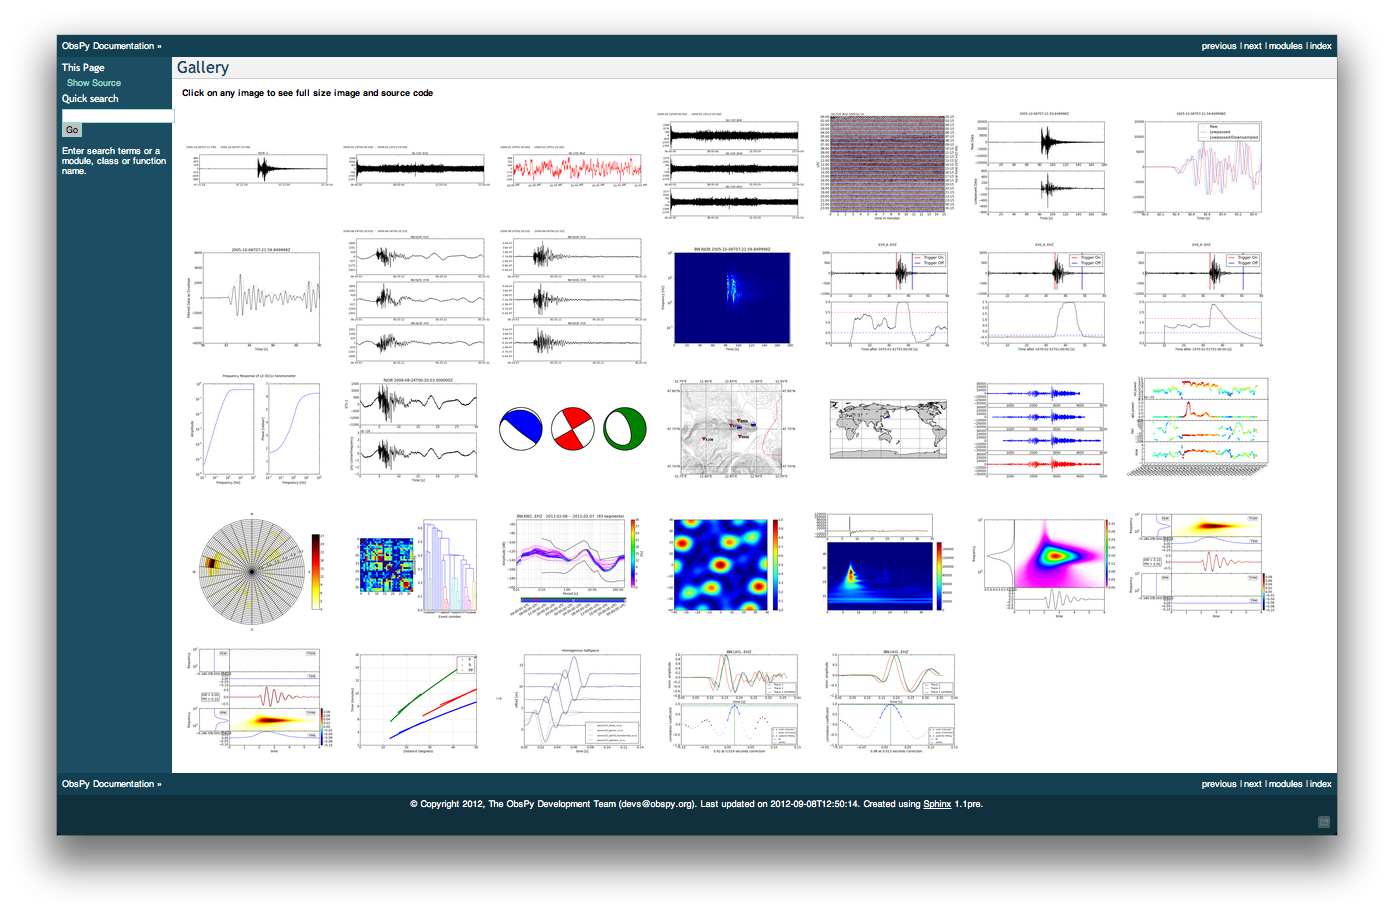
\includegraphics[width=\textwidth]{./gallery.png}
\end{frame}



\begin{frame}[plain]{Installing ObsPy}
    \begin{itemize}
        \item \textbf{Debian/Ubuntu} - via package management (https://deb.obspy.org)
        \item \textbf{Windows} - Windows installer (automatically installs all dependencies)
        \item \textbf{OSX $\ge$ 10.6} - one-click-install application (contains all dependencies)
    \end{itemize}
    For the most recent additions and bug fixes install the developer version.

    \vspace{2em}

    Detailed instructions for all platforms can be found on \textbf{www.obspy.org}.
\end{frame}


\begin{frame}[plain]{}
    \begin{center}
        \textcolor{lmu@darkgreen}{\LARGE{Thanks for your attention.}}
    \end{center}
\end{frame}


\end{document}
